\section{Background}

When discussing the `digital fitness' of languages \cite{soria2016fostering}
with respect to their usage, dissemination and accessibility on the web, resp., of web resources for speakers of that languages, emphasis is often put on parameters such as the size of the speaker community and the number (or existence) of resources and tools. We consider this perspective, however, to be a little bit too narrow, in that the existence of, say, spell checkers, chatbots, MT technology, dictionaries or just plain texts may not be equally helpful to all speakers of the language under consideration, depending on the \emph{degree of internal diversity} of the language, the orthographies used to write its dialects, and the degree of standardization accepted by the speaker community. As a point in case, we describe an approach for creating both a machine-readable dictionary and interdialectal links for Low German (Low Saxon, ISO 639-2 \code{nds}), a European minority language with a high degree of phonological, morphological and orthographic diversity. It is to be noted that, although Modern Low German has developed a vibrant production of (regional) literature since about 1800, it not only lacks a written standard, but also corpora, machine-readable dictionaries, and interdialectal dictionaries. More importantly, it also has a deficit of parallel texts, and in particular, texts attested in more than one variety of Low German, so that most modern NLP technology tailored towards exploiting parallel text are not applicable. Likewise, there is a problem in applying off-the-shelf embeddings or LLMs due to the lack of consistent training data on the web.\footnote{
    We are aware of only one larger-scale experiment with using LLMs for Low German. According to public reports, however, this largely failed to achieve its preliminary goals after a 6 month piloting period, and was abandoned in August 2024, cf. \url{https://www.ndr.de/kultur/norddeutsche_sprache/niederdeutsch/Pepper-Blog-34-Neue-wissenschaftliche-Wege,pepperblog180.html}.
}

Without artifically enforcing normalization and standardization, what is needed to develop effective NLP support for Low German is a digital Rosetta stone that allows us to leverage materials from different language varieties and to access them in a uniform way. This can by done by means of language normalization, but this has been a controversial topic in the past \cite{Christiansen1975}, and -- beyond the level of geographically confined regions -- seems to be largely rejected by the speaker community. Instead, we focus on technologies to create `non-invasive' synergies between dialect-specific resources on the web, by creating links between regional dictionaries, and by providing a mapping routine capable to \emph{spot} formally corresponding words in different dialects which can subsequently be linked. In this paper, we primarily focus on the first aspect, on providing adequate methods of access to such data for both humans and machines. On the one hand, web-scale linking across physically dispersed data sources can be naturally addressed by means of RDF and Linked Open Data technology \cite{cimiano-et-al-2020-lld-intro}, but providing our data as Linguistic Linked Open Data (LLOD) involves a number of technological challenges in data modelling (of the dictionaries and inter-dictionary links), in accessibility (i.e., readability for a human), and also in terms of legal constraints (in fact, most dictionaries freely accessible over the web adopt a proprietary licensing model so that their content cannot be directly used -- but it can be linked).

Low German or Low Saxon (self-designation \word{Plattdüütsch}, \word{Nedersassisch} or \word{Nedersaksisch}) is a West Germanic language historically spoken in northern Germany, the Netherlands and the southern coast of the Baltic Sea. It is closely related to and has been in continuous contact with Dutch, High German and Frisian, but it followed its own developmental trajectory since its first recorded texts (esp., a 9th c. gospel harmony).

. It is thus recognized as a regional language and protected under the European Charter for Regional or Minority Languages (ECRML). 
Historically, (Middle) Low German was a major language of trade and administration, particularly during the Hanseatic League (13th–17th centuries), when it served as a lingua franca across the North and Baltic Sea regions. However, its status declined, with High German (in Germany) and Dutch (in the Netherlands) replacing it as the dominant language of education, administration, and media. Today, Low German is considered threatened (vulnerable) \cite[p.25]{moseley2010atlas}, and the 19th and 20th c. have seen younger generations increasingly shifting to the respective national languages. While it still has millions of passive speakers, active speakers are far fewer and to a large extent senior citizens \cite{AdlerEhlersGoltzetal.2019}, so that one of the most pressing issues facing Low German today is the transmission challenge to the next generation of speakers. This includes didactic and educational material, but also basic NLP tools like spell checkers, machine translation, speech recognition, and text-to-speech systems are either completely absent or in very early stages of development. A major challenge here is the fragmentation of the modern dialects of Low German, which diverged greatly since the middle ages, both in their phonology and their grammar. Individual dialects are primarily defined by their distinct and specific development of Middle Low German vowels, with regional changes in their quality (esp., diphthongization and monophthongization processes) and quantity (length). Some, mostly northern, dialects lost the unvoiced vowels of Middle Low German (and, as a result, abandoned large swaths of their nominal and verbal morphology), while others retained them (along with the four case nominal morphology and the subjunctive present). Whereas this north-south division is the result of developments that occurred mostly between 1600 and 1850, there also exists an west-east division that reflects the eastwards expansion of Low German during the Middle Ages, with Western dialects spoken in the same area as Old Saxon (and morphologically marked by a uniform verbal plural in \word{-(e)t}) and Eastern dialects spoken in the area that was colonized after the 12th c. (and morphologically marked by a verbal plural in \word{-en}). Although the dialects east of the river Oder effectively ceased to be spoken after WWII, (Eastern) Low German persists in emmigrant varieties originally spoken in areas in modern Poland (Pomerano, a regionally recognized minority language in Brazil), Ukraine and Russia (Plautdietsch, primarily spoken by the Mennonite diaspora in the Americas). 
As a result of this particularization, there is no accepted standard variety, and, in fact, this has been acknowledged in information technology by awarding different regional varieties of Low German (ISO 639-2 language code \code{nds}) their own ISO 639-3 identifiers (see Tab. \ref{tab-dialects-and-isocodes} for the major varieties being spoken today). This technological gap makes it difficult to use Low German in digital communication, reducing its visibility and usability in the modern world. The absence of NLP tools also hinders academic research, automated language processing, and efforts to create digital content in Low German. 

\begin{table}
    \centering
    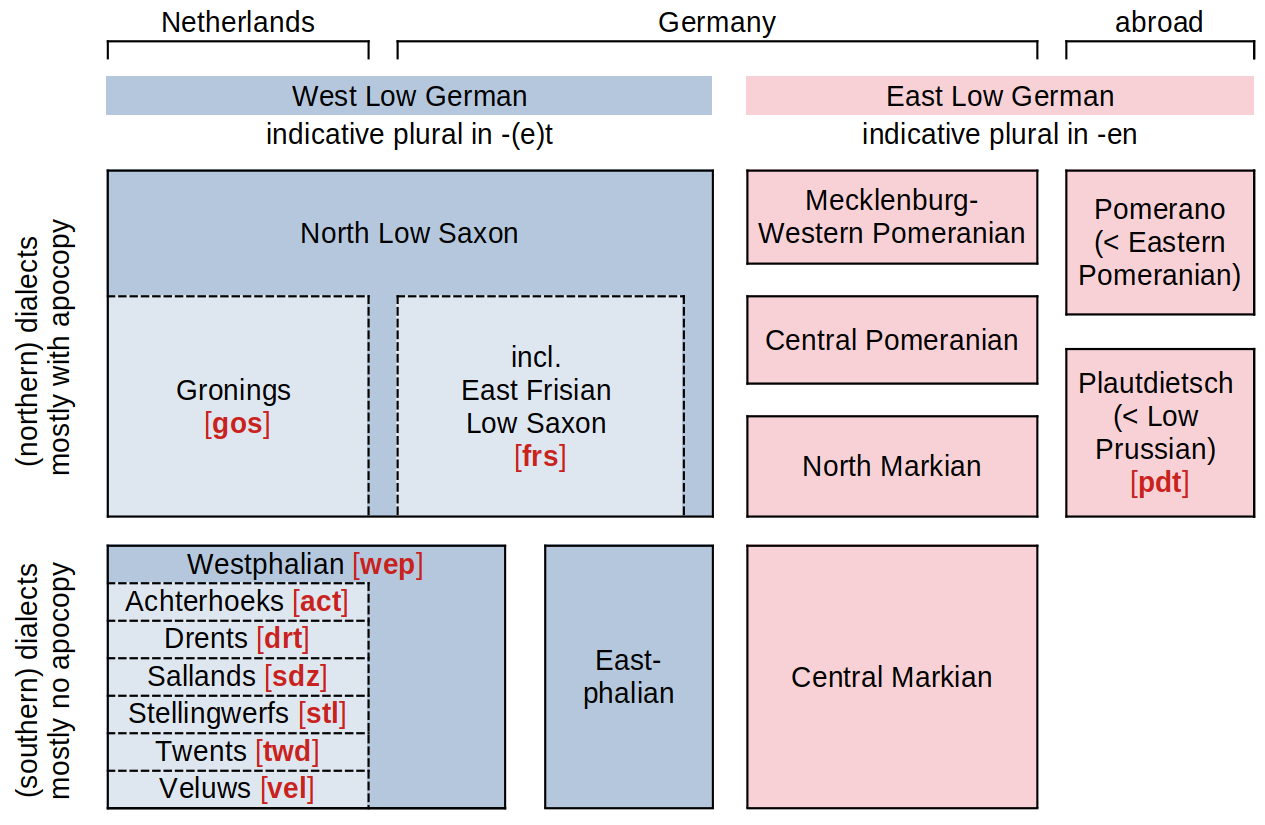
\includegraphics[width=1.0\linewidth]{img/dialects-and-iso632-codes.png}
    \caption{Major dialects of Low German (ISO 639-2 \code{nds}), with regional ISO 639-3 codes in red square brackets.}
    \label{tab-dialects-and-isocodes}
\end{table}

Despite its challenges, Low German enjoys cultural and regional recognition. Efforts to revitalize the language include educational programs, literature, radio broadcasts, and online initiatives. However, without stronger support on many levels, the survival of Low German as a living language remains uncertain. In fact, social networks and digital language resources may play a role in transmission and revitalization of the Low German language, and indeed, this is what we see for other minority languages all over the world. 
To preserve Low German, more work is needed to integrate it into digital spaces. Developing NLP tools, expanding online resources, and increasing its presence in modern media are crucial steps in ensuring that Low German remains a functional and thriving language for future generations. At the moment, however, even the most basic NLP resources are still lacking. For Low German, only small samples of annotated major corpora are known to exist, no parallel corpora (although translated texts can be found, mostly translated into Low German), and no machine-readable dictionaries. 

A \emph{machine-readable dictionary (MRD)} is a structured lexical resource designed for computational use rather than human readability. Unlike traditional dictionaries, MRDs are formatted in a way that allows software applications to process and analyze linguistic data efficiently. They store information such as word meanings, grammatical properties, pronunciations, and translations in a structured manner to facilitate the development of downstream applications. For low-resource languages, \emph{machine-readable dictionaries} (MRDs) play a crucial role in developing foundational NLP technologies. In particular, this is the case for language varieties that have been the subject of linguistic research in the past (so that word lists or dictionaries are available), but that have been largely neglected by NLP or corpus linguistics (so that no digital corpus data is available). This paper addresses the development of an initial set of MRDs for different varieties of Low German. 
Despite being a literary language for about a thousand years and an extant regional literature from the 19th and 20th c., this is the case for Low German: Textual material is available, but not in digital form. Since low resource languages lack large annotated corpora, extensive linguistic databases, or pre-trained models, MRDs serve as a primary data source for computational applications. They facilitate the creation of essential tools such as spell checkers, part-of-speech taggers, and lemmatizers, helping bridge the technological gap between widely spoken and endangered languages. We can build on a number of digital dictionaries in existence, but each pertains to a different variety and all are designed for human consumption, and not for subsequent use in natural language processing. In addition to that, most of these are copyright-protected, either explicitly or by default copyright (if copyright is undeclared). The approach we suggest can, however, be applied to other Low German dictionaries and dialects if copyright can be secured.
    
A key technology for building structured and interoperable MRDs is \emph{OntoLex-Lemon}, an RDF (Resource Description Framework) vocabulary  designed for representing lexical and semantic data on the web. OntoLex allows lexicons to be linked to external knowledge bases and other linguistic resources, enhancing interoperability. It uses, RDF, a W3C standard, to provide a flexible, graph-based data model that enables rich semantic annotations and structured linguistic relationships. Together, these technologies ensure that dictionaries for low-resource languages are not isolated but can be \emph{integrated into broader linguistic ecosystems}, facilitating cross-linguistic research and NLP. By leveraging OntoLex and RDF, MRDs for low-resource languages can be built in a way that supports automated processing, encourages digital preservation, and enables their incorporation into modern NLP applications. These technologies make it easier to link lexical resources across languages, ensuring that low-resource languages gain better representation in computational linguistics and digital tools. As such, OntoLex has been a cornerstone for integrating lexical data into the Linguistic Linked Open Data (LLOD) cloud. 

The \emph{Linguistic Linked Open Data (LLOD)} cloud is a structured network of interlinked linguistic resources published in accordance with the principles of Linked Data \cite{bizer2009linked}. It provides a semantic web-based infrastructure for representing and integrating linguistic data, including lexicons, corpora, terminologies, and ontologies. By leveraging RDF (Resource Description Framework) and related technologies, the LLOD cloud enables interoperability and data exchange across various NLP and linguistic applications \cite{chiarcos2013linguistic}.  A key advantage of the LLOD approach is its ability to connect diverse linguistic datasets, making them accessible for computational use. Resources such as OntoLex-Lemon facilitate the representation of lexicons, while linguistic ontologies like OLiA (Ontologies of Linguistic Annotations) provide standardized annotation frameworks \cite{chiarcos2012olia}. The LLOD cloud benefits low-resource languages by linking their limited linguistic data to richer datasets, fostering NLP development and linguistic research. By structuring linguistic resources using open standards, the LLOD cloud contributes to the creation of multilingual and interoperable NLP systems, supporting tasks such as machine translation, semantic search, and corpus analysis. As the LLOD cloud expands, it plays an increasingly vital role in the digital preservation and computational accessibility of linguistic knowledge.  


%digital and digital-born Low German dictionaries

%Selected digital dictionaries

%\begin{itemize}
%    \item https://woerterbuchnetz.de/?sigle=WWB&lemid=A00001
%    \item Digitales Wörterbuch Niederdeutsch (dwn), https://www.niederdeutsche-literatur.de/dwn/
%    \item https://www.ndr.de/kultur/norddeutsche_sprache/plattdeutsch/woerterbuch101.html: unregulated orthographies
%    \item Plattmakers
 %   \item https://www.platt-wb.de/
  %  \item WöWö
   % \item Mittelelbisches (nur A-O, https://mew.uzi.uni-halle.de/artikel/25748)
    %\item https://www.plattdeutsches-woerterbuch.de/search (suche nach leerem string, um alles zu bekommen), keine einzelseiten
%    \item https://netz.sass-platt.de/hoch-platt
%    \item wiktionary
%\end{itemize}

A number of digital, and in parts, digital-born, dictionaries of different varieties of Low German are available online. As far as Germany is concerned, the only digital Low German dictionary with a permissive license we are aware of is Wiktionary, a collaborative, crowd-sourced dictionary covering multiple languages, including Low German. Includes definitions, pronunciation guides, etymology, and translations. As a crowd-sourced resource, it lacks standardization, as different sets of orthographic conventions are applied by different contributors. Another, digital-born dictionary -- although only available in MS Office and PDF formats -- is Wöhrner Wöör (WöWö), a Low German dictionary for the Dithmarschen variety of North Low Saxon by Peter Neuber, originally published in print in 2001, but subsequently published as PDF and MS Office documents only.\footnote{\url{https://ditschiplatt.de/woehrner-woeoer/}} 
With permission of the author, % WHICH WE DON'T HAVE YET
we use this as the basis for our efforts.

Other digital dictionaries of Low German are available under restrictive (or implicit, i.e., restrictive-by-default) licenses include the following:

\begin{description}
\item[Sass’ Plattdeutsches Wörterbuch] (\href{https://netz.sass-platt.de/hoch-platt}{Sass-Netz})  
    Based on Johann Sass' Plattdeutsch dictionary, which defines a standardized spelling system. Provides High German → Low German translations and is one of the most widely accepted spelling systems for written Plattdeutsch, albeit a deficient one (several sounds are systematically conflated) that also is not applicable to all varieties. In particular, the orthography lacks support for Westphalian, Eastphalian and Central Markian, whereas northern varieties (esp., North Low Saxon) can be represented more or less faithfully. Copying is explicitly restricted to private, non-commercial use. We assume that this also rules out academic usage.

\item[Digitales Wörterbuch Niederdeutsch (DWN)] is a collection of digital Low German dictionaries covering multiple dialects.\footnote{\url{https://www.niederdeutsche-literatur.de/dwn/}} It seems to be developed and maintained by a single individual only, albeit in parts in collaboration with academic partners (e.g., the Kompetenzzentrum für Niederdeutschdidaktik of the University of Greifswald, for whose Mecklenburgian dictionary it provides the technical backbone).\footnote{\url{https://länderzentrum-für-niederdeutsch.de/renate-hermann-winter-woerterbuch-nun-online/}} The dictionaries are searchable and provide semi-structured HTML content. No explicit license is given, thus restricted copyright. It should be noted, however, that the original copyright of several dictionaries provided via DWN has expired. Yet, database right applies to the digital edition. Aside from an all-over Low German dictionary compiled from diverse sources, it also provides regional dictionaries.

\item[Westfälisches Wörterbuch (WWB)] is a comprehensive academic dictionary of Westphalian, as spoken in northwestern Germany, made available as part of the Wörterbuchnetz platform \cite{wwb}.\footnote{\url{https://woerterbuchnetz.de/}}. It provides detailed historical and etymological information in semi-structured HTML. The Wörterbuchnetz also provides an API access, although only to lemma lists and full text search, not to the actual entries. No explicit license is given, thus restricted copyright.

\item[NDR Plattdeutsch Wörterbuch] aims to be a general Low German dictionary and is hosted by Norddeutscher Rundfunk (NDR).\footnote{\url{https://www.ndr.de/kultur/norddeutsche_sprache/plattdeutsch/woerterbuch101.html}} Most of its content seems to be crowd-sourced, it thus contains unregulated orthographies, so that words appear in varying spellings or for different dialects. Focuses on practical and everyday vocabulary rather than linguistic precision. No explicit license is given, thus restricted copyright.

\item[Plattmakers] \href{https://plattmakers.de} is a collaborative online Low German dictionary, similar to Wiktionary, based on a digital-born multi-dialectal core dictionary developed by Marcus Buck in 2009. It covers all Low German dialects, providing translations in German, Dutch, and English. Lemmas are normally given in North Low Saxon or normalized to a North Low Saxon pronounciation. Words include regional maps, explanations in Low German, and cognates in High German, English and Dutch. Without an explicit license statement, the content is copyright-protected.

\item[Online-Wörterbuch für ostfriesisches Plattdeutsch] (\href{https://www.platt-wb.de/}) 
    is a dictionary portal that provides search over a dictionary for East Frisian Low German, compiled from various sources and edited by the Plattdüütskbüro der Ostfriesischen Landschaft. The dictionary is free searchable for German and Low German in both directions, and support partial matches. Without explicit license statement, it is copyright-restricted.

\item[Mittelelbisches Wörterbuch] (\href{https://mew.uzi.uni-halle.de/artikel/25748}{MEW})
    A dictionary of Middle Elbe Low German, currently covering only A–O. Subject of an ongoing linguistic research project based at the University of Halle.  The dictionary is published under CC BY-NC-ND. We interpret the ND clause as prohibiting the conversion to a Linked Data representation.

\item[Platt för Plietsche; Plattdeutsch Übersetzer für Schleswig-Holstein, Hamburg, Bremen und Teilbereiche von Mecklenburg-Vorpommern und Niedersachsen] (\href{https://www.plattdeutsches-woerterbuch.de/}) provides search over a bilingual German-Low-German word list. Without explicit license statement, this is copyright-protected.



\end{description}

Major dictionaries available in print (or PDF) only include the Berlin-Brandenburg dictionary, the Niedersächsisches Wörterbuch, the Pommersches Wörterbuch, the Schleswig-Holsteinisches Wörterbuch \cite{mensingotto}. The Wossidlo-Teuchert dictionary of Mecklenburgian is currently in the process of integration into Wörterbuchnetz.\footnote{\url{https://www.germanistik.uni-rostock.de/personen/professuren/prof-dr-andreas-bieberstedt/projekte-und-forschungsschwerpunkte/wossidlo-teuchert-online/}}

More dictionaries:
- Das Niedersächsische Wörterbuch ist bislang ebenfalls nur in print verfügbar und nur bis zum buchstaben s veröffentlicht, vgl. https://www.uni-goettingen.de/de/publikationen/219293.html



As for machine-readable dictionaries of Low German, we are not aware of any Low German lexical datasets except for Low German terms in foreign-language editions of DBnary, i.a., the database edition of the Wiktionary, also cf. ACoLi dictionary graphs. However, PanDoc data is generally of mixed quality, as it is largely based on automated OCR. Wiktionary data is crowdsourced, and for a language without a written standard, this data is too unsystematic to be used and reliably linked with other lexical resources, as it freely mixes mixes regional and author-specific orthographies.

In addition to these dictionaries, there are many print dictionaries, also in the public domain, but not reliably digitized.

